

\documentclass[oneside,20pt]{article}          % please do not change
\usepackage[b5paper]{geometry}	    % your paper can be easily printed on a4 or letter paper with enlargenment      
                                    % comment if you have problem with print     
\usepackage{amsfonts,amsmath,latexsym,amssymb}
\usepackage{graphicx}
%%% remove comment delimiter ('%') and specify parameters if required
%\usepackage[dvips]{graphics}

\begin{document}

%%% remove comment delimiter ('%') and select language if required
%\selectlanguage{spanish} 

\noindent 
\begin{center}
  \texttt{LABORATOR 3-- Socket Programming în Python.}        
\end{center}

\section{Socket Programming}
\noindent                 
\\\\\
Programarea socketului este o modalitate de a conecta două noduri dintr-o rețea pentru a comunica între ele. Un socket (nod) ascultă pe un anumit port la un IP, în timp ce celălalt ajunge pentru a forma o conexiune. Serverul joacă rolul de ascultător în timp ce clientul are legătura la server.
Ele sunt adevăratele coloane vertebrale din spatele navigării pe web. În termeni mai simpli, există un server și un client.
Programarea socketului este începută prin importul bibliotecii de socket și realizarea unui socket simplu.

\begin{center}
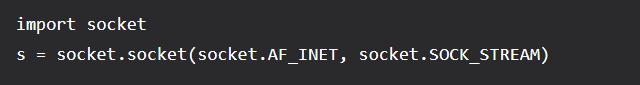
\includegraphics[height = 1 cm]{0.png}
\end{center}

Aici am făcut o instanță de socket și i-am transmis doi parametri. Primul parametru este $AF\_INET$, iar al doilea este $SOCK\_STREAM$. $AF\_INET$ se referă la adresa-familiei ipv4. $SOCK\_STREAM$ înseamnă protocol TCP orientat spre conexiune.
Acum ne putem conecta la un server folosind acest socket.\\
Conectarea la un server:\\

\begin{center}
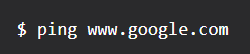
\includegraphics[height = 1 cm]{0.1.png}
\end{center}
Rețineți că, dacă apare vreo eroare în timpul creării unui socket, atunci avem o eroare și ne putem conecta la un server doar cunoscând IP-ul acestuia. Puteți găsi IP-ul serverului folosind aceasta:


\begin{center}
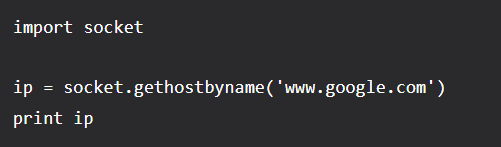
\includegraphics[height = 2 cm]{0.2.png}
\end{center}

Un alt exemplu de script pentru conectarea la google:


\begin{center}
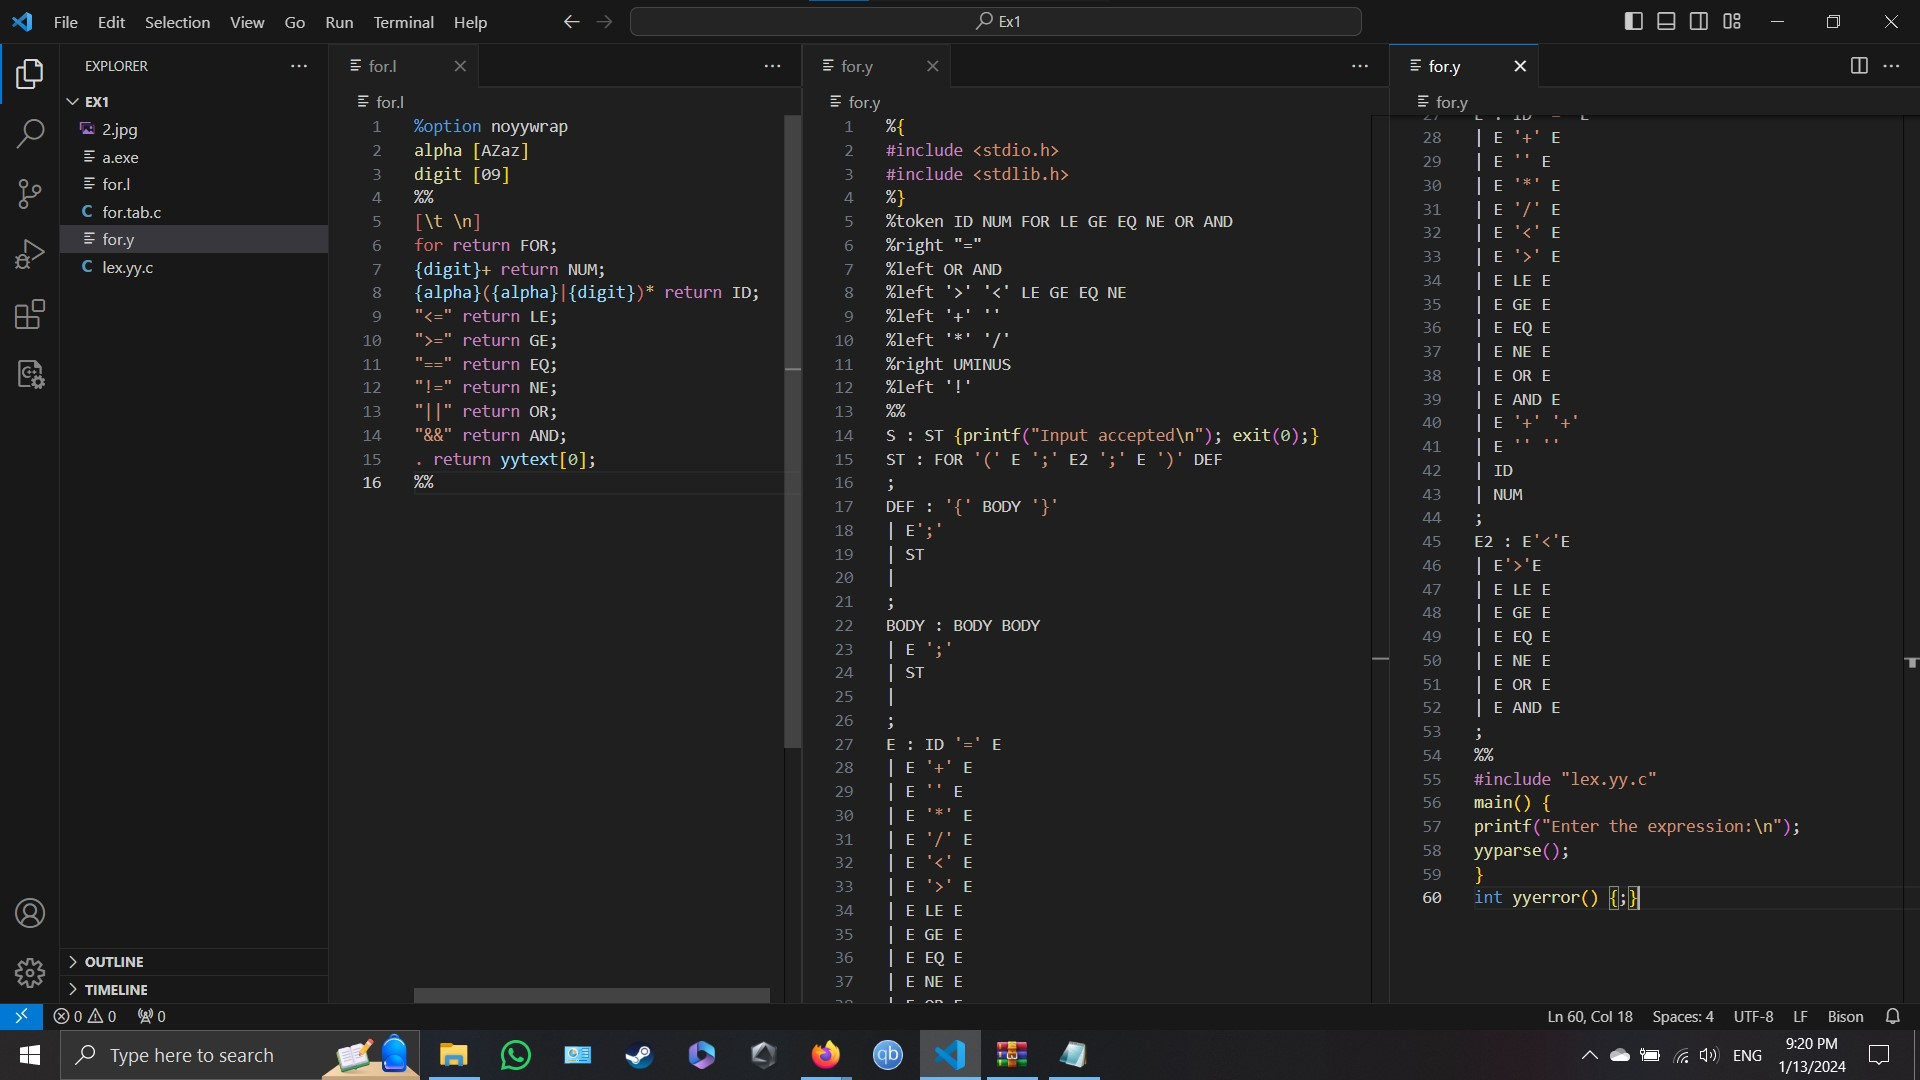
\includegraphics[height = 6 cm]{1.png}
\end{center}
la Output va afisa:
\begin{center}
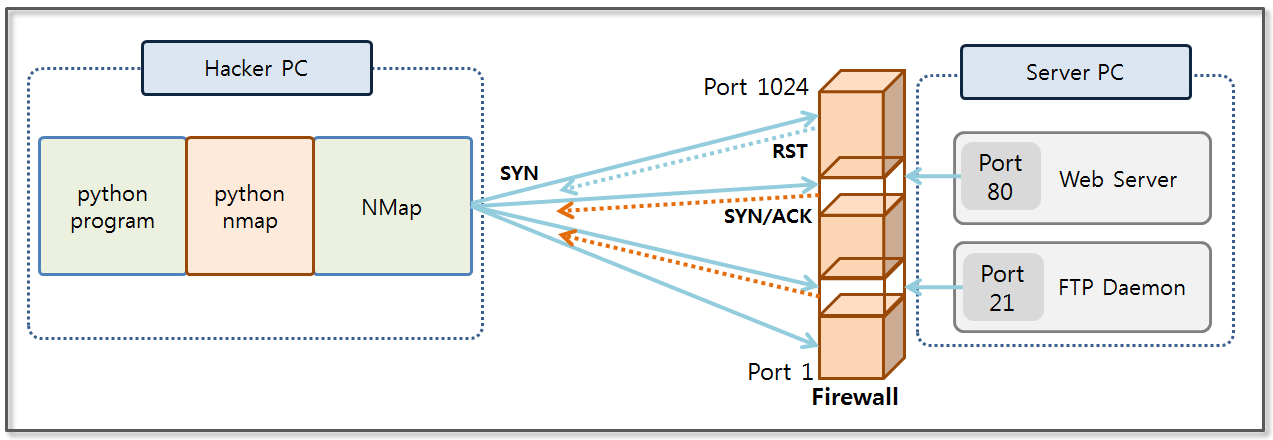
\includegraphics[height = 1 cm]{2.png}
\end{center}

 Să concluzionăm: În primul rând, am realizat un socket.\\
Apoi am rezolvat IP-ul google și, în sfârșit, ne-am conectat la google.\\
Acum trebuie să știm cum putem trimite niște date printr-un socket.\\
Pentru trimiterea datelor, biblioteca socket are o funcție sendall. Această funcție vă permite să trimiteți date către un server la care este conectat și serverul poate trimite și date către client folosind această funcție.\\
Un program simplu server-client:\\

 \begin{center}
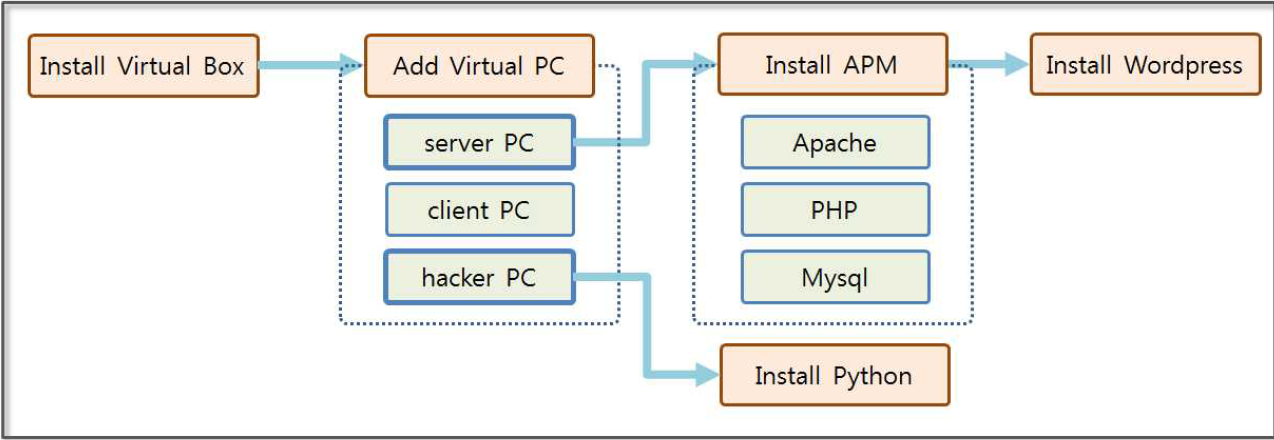
\includegraphics[height = 5 cm]{3.png}
\end{center}
Server :

Un server are o metodă bind() care îl leagă la un anumit IP și port, astfel încât să poată asculta cererile primite pe acel IP și port. Un server are o metodă listen() care pune serverul în modul de ascultare. Acest lucru permite serverului să asculte conexiunile primite. Și, în sfârșit, un server are o metodă accept() și close(). Metoda accept inițiază o conexiune cu clientul, iar metoda close închide conexiunea cu clientul.\\
În primul rând, importăm socketul necesar.
Apoi am făcut un obiect socket și am rezervat un port pe computerul nostru.
După aceea, ne-am conectat serverul la portul specificat. Trecerea unui șir gol înseamnă că serverul poate asculta conexiunile primite și de la alte computere. Dacă am fi trecut de 127.0.0.1, atunci ar fi ascultat doar acele apeluri efectuate în computerul local.
După aceea punem serverul în modul de ascultare.5 aici înseamnă că 5 conexiuni sunt menținute în așteptare dacă serverul este ocupat și dacă un al 6-lea socket încearcă să se conecteze atunci conexiunea este refuzată.
În cele din urmă, facem o buclă și începem să acceptăm toate conexiunile de intrare și să închidem acele conexiuni după un mesaj de mulțumire către toate socketurile conectate.
Client:
Acum avem nevoie de ceva cu care un server poate interacționa. Am putea da telenet la server astfel doar pentru a ști că serverul nostru funcționează. Tastați aceste comenzi în terminal:
 \begin{center}
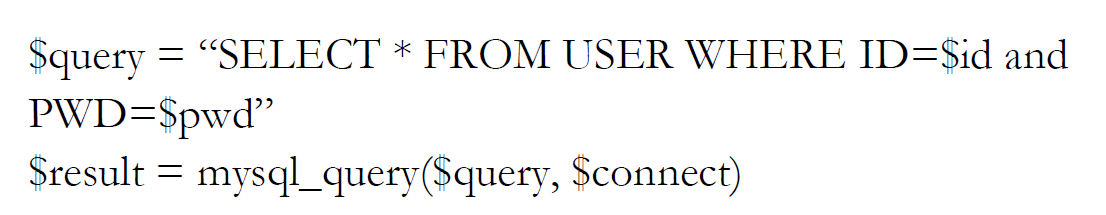
\includegraphics[height = 5 cm]{4.png}
\end{center}

Dacă ”telnet” nu este recunoscut, pe Windows, căutați funcțiile Windows și activați caracteristica ”client telnet”.\\
Ieșire:\\

 \begin{center}
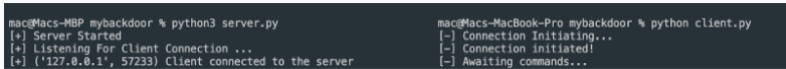
\includegraphics[height = 4 cm]{6.png}
\end{center}
Aceasta arata că serverul nostru funcționează.
Acum pentru partea clientului:
 \begin{center}
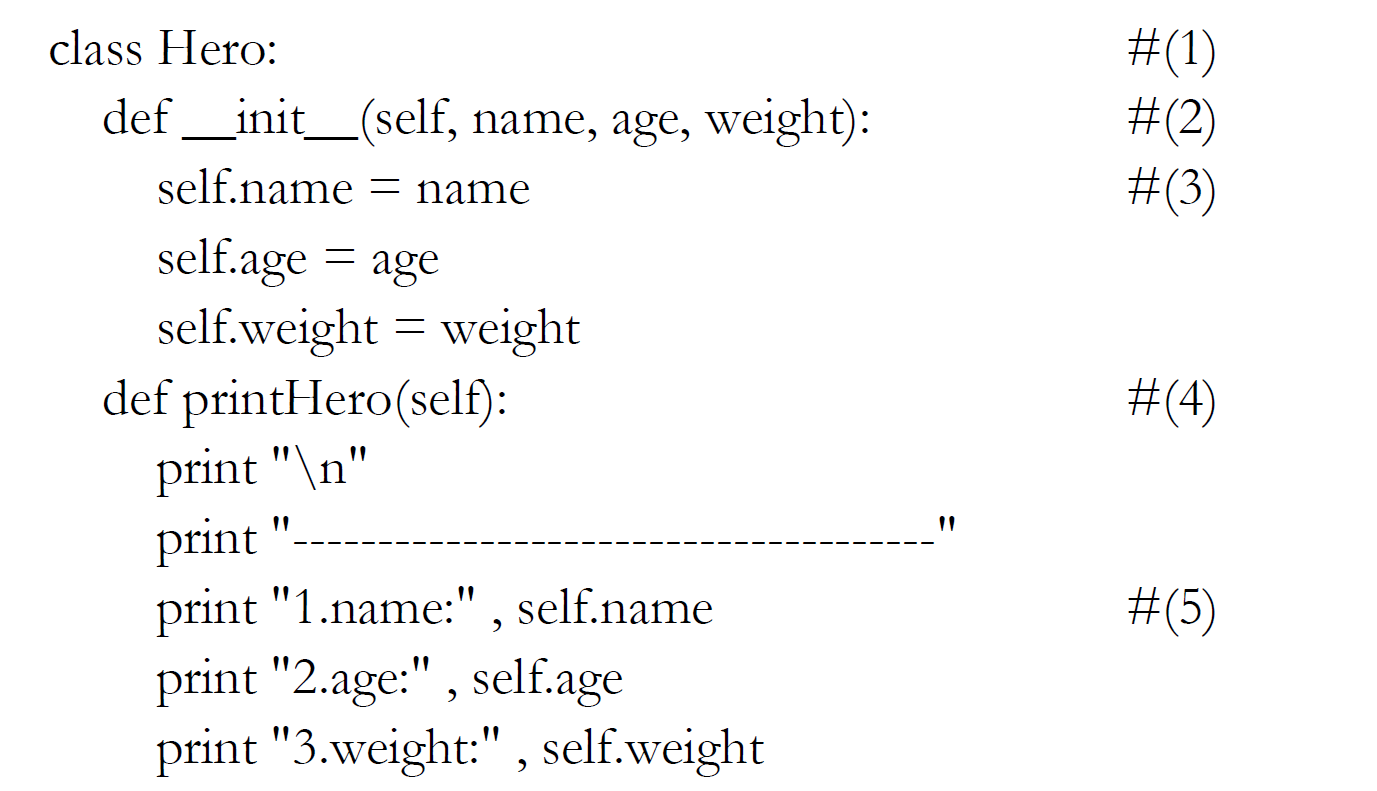
\includegraphics[height = 4 cm]{7.png}
\end{center}

În primul rând, facem un socket.\\
Apoi ne conectăm la localhost pe portul 12345 (portul pe care rulează serverul nostru) și, în sfârșit, primim date de la server și închidem conexiunea.\\
Acum salvăm acest fișier ca și client.py și rulăm de pe terminal după pornirea scriptului de server.\\

\section{Steganografie cu Python}
Steganografia imaginii este procesul de ascundere a datelor secrete într-o imagine. În această postare, vom ascunde o imagine în alta și o vom converti într-o altă imagine și apoi vom extrage înapoi ambele imagini din imaginea anterioară.

Ideea din spatele steganografiei bazate pe imagini este foarte simplă. Imaginile sunt compuse din date digitale (pixeli), care descrie ceea ce este în interiorul imaginii, de obicei culorile tuturor pixelilor. Din moment ce știm că fiecare imagine este formată din pixeli și fiecare pixel conține 3 valori (roșu, verde, albastru).

De exemplu, să presupunem că trebuie să ascundem img2 în img1, unde ambele img1 și img2 sunt date ca matrice de valori pixeli. Dimensiunea img2 trebuie să fie mai mică decât dimensiunea img1. Folosim imagini color, prin urmare ambele vor avea 3 valori (roșu, verde, albastru). Valoarea fiecărui pixel variază de la 0 la 255, deci valoarea fiecărui pixel este de 1 octet sau 8 biți. Fie img[i][j][l] valoarea pixelului la locația (i, j) și a canalului l unde i variază de la 0 la lățime și j variază de la 0 la înălțime și l variază de la 0 la 2.


Notă: Calitatea noilor imagini este puțin mai mică decât a imaginilor vechi.
Dorim să ascundem imaginea 2 în imaginea 1. Mai jos este implementarea in Python.
 \begin{center}
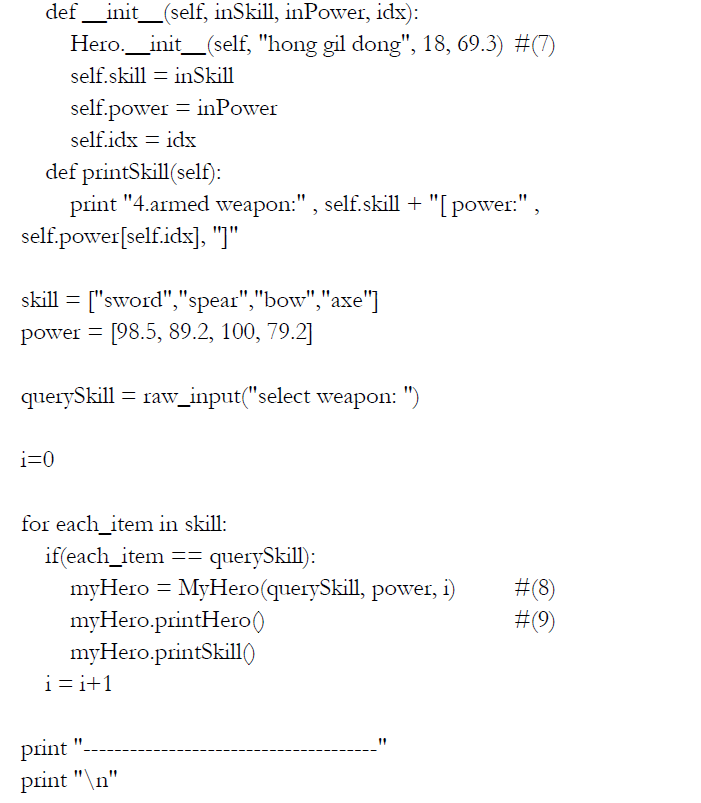
\includegraphics[height = 5 cm]{8.png}
\end{center}
 \begin{center}
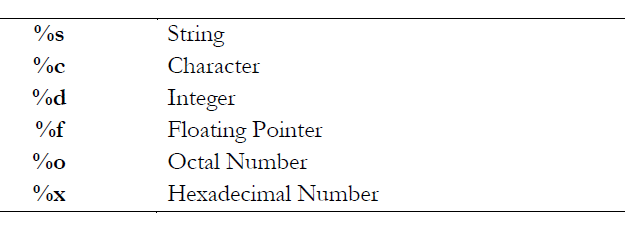
\includegraphics[height = 4 cm]{9.png}
\end{center}
 \begin{center}
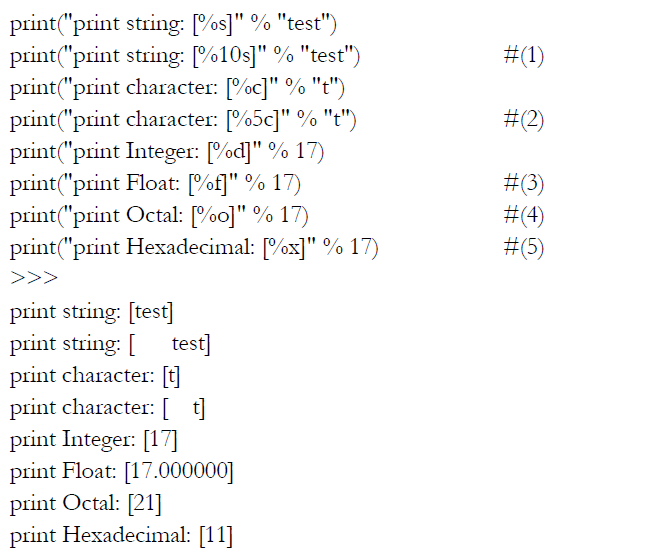
\includegraphics[height = 3 cm]{10.png}
\end{center}
\section{Steganografie bazată pe imagini folosind Python}
1) Criptare

Abordare:

Importați imaginea din modulul PIL folosind cuvântul cheie import.\\
Importați modulul stepic folosind cuvântul cheie import.\\
Deschideți imaginea folosind funcția open() a modulului Image, pasând numele/calea fișierului imagine ca argument în care va fi stocat mesajul secret.\\
Dați un mesaj secret aleatoriu și stocați-l într-o variabilă.\\
Convertiți mesajul secret dat de mai sus în format UTF-8 folosind funcția encode() și stocați-l în aceeași variabilă.\\
Treceți imaginea dată și mesajul secret în funcția encode() a modulului stepic care oferă o nouă imagine în care mesajul secret este ascuns.\\
Salvați imaginea codificată/criptată de mai sus cu un nume și o extensie aleatorie folosind funcția save().
Tipăriți un text aleatoriu pentru confirmare.\\
Ieșirea din program.\\
Mai jos este implementarea:

 \begin{center}

\includegraphics[height = 4 cm]{11.png}
\end{center}
2) Decriptare\\

Abordare:\\

Importați imaginea din modulul PIL folosind cuvântul cheie import.\\
Importați modulul stepic folosind cuvântul cheie import.\\
Deschideți imaginea din care doriți să extrageți mesajul secret (imaginea criptată) folosind funcția open() pasând numele fișierului/calea ca argument.\\
Stocați-l într-o variabilă.\\
Treceți imaginea criptată de mai sus la funcția decode() a modulului stepic pentru a oferi mesajul secret criptat în format șir.\\
Stocați-l într-o altă variabilă.\\
Tipăriți un text aleatoriu pentru confirmare.\\
 Imprimați mesajul decriptat/decodificat.\\
Ieșirea din program.\\
 \begin{center}
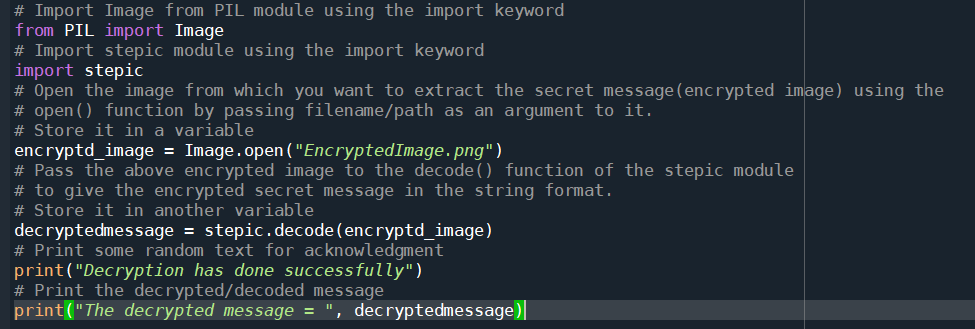
\includegraphics[height = 4 cm]{12.png}
\end{center}
 Se va vedea la decodificare mesajul ascuns de noi in prealabil la codificare.
\section{Bibliografie}
Python Hacking Essentials Paperback 2015 by Earnest Wish, \\
https://www.amazon.com/Python-Hacking-Essentials-Earnest-Wish/dp/1511797568\\
https://www.geeksforgeeks.org/socket-programming-python/


\end{document}
